\subsection{Turning Waves: Crafting Circular Polarization with Yagi Antennas!}

\begin{tcolorbox}[colback=gray!10, colframe=black, title=E9D02] How can two linearly polarized Yagi antennas be used to produce circular polarization?
\begin{enumerate}[label=\Alph*.]
    \item Stack two Yagis to form an array with the respective elements in parallel planes fed 90 degrees out of phase
    \item Stack two Yagis to form an array with the respective elements in parallel planes fed in phase
    \item \textbf{Arrange two Yagis on the same axis and perpendicular to each other with the driven elements at the same point on the boom and fed 90 degrees out of phase}
    \item Arrange two Yagis collinear to each other with the driven elements fed 180 degrees out of phase
\end{enumerate} \end{tcolorbox}

\subsubsection*{Concepts Involved}

To understand how two linearly polarized Yagi antennas can produce circular polarization, it is crucial to comprehend the concepts of polarization, phase difference, and antenna arrangement.

1. \textbf{Linear Polarization:}: A Yagi antenna typically has a directional radiation pattern and is linearly polarized, meaning it radiates electromagnetic waves in a single plane.

2. \textbf{Circular Polarization:}: For an antenna system to produce circular polarization, the two components of the polarization must be 90 degrees out of phase. This means that one component must have a different phase than the other by exactly a quarter of a wavelength.

3. \textbf{Antenna Arrangement:}: By arranging two Yagi antennas such that they are perpendicular to each other (one oriented horizontally and the other vertically) and feeding them with a phase difference of 90 degrees, circular polarization is achieved. 

    - In the correct option (C), the Yagis are arranged on the same axis and are fed 90 degrees out of phase. This ensures that as one antenna reaches its maximum in one plane, the other is at zero, thereby creating the conditions necessary for circular polarization.

\subsubsection*{Calculations and Diagram Representation}

While specific calculations relating to wave propagation and antenna gain are not directly involved in this question, we can outline the concept of phase difference.

- \textbf{Phase Difference Calculation:}: 
    - For creating circular polarization, we need a phase shift of \(90^\circ\). This can be achieved by using a phase shifter or a delay line in the feed system of the second antenna.

\begin{center}
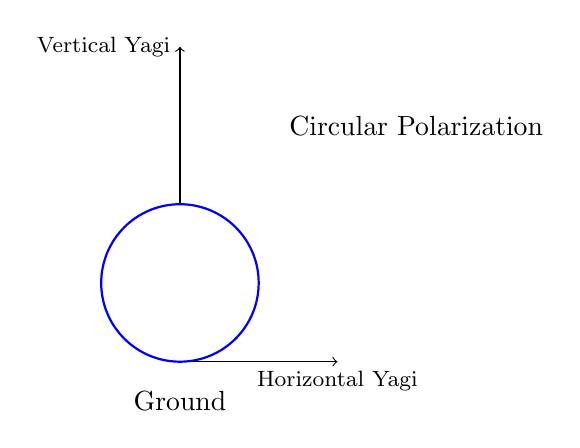
\begin{tikzpicture}
    % Draw the two Yagi antennas
    \draw[->] (0,0) -- (2,0) node[anchor=north] {\footnotesize Horizontal Yagi};
    \draw[->] (0,2) -- (0,4) node[anchor=east] {\footnotesize Vertical Yagi};
    
    % Draw a circular wave to represent circular polarization
    \draw[blue, thick] (1,1) arc[start angle=0, end angle=360,radius=1cm];
    
    % Labels
    \node at (0,-0.5) {Ground};
    \node at (3,3) {Circular Polarization};
\end{tikzpicture}
\end{center}

In summary, to produce circular polarization with two Yagi antennas, we arrange and feed them appropriately while ensuring they are perpendicular, which entails knowledge of antenna properties and the physics of electromagnetic wave propagation.